
\documentclass[a4paper,12pt]{article}
\usepackage[ngerman]{babel}
% \usepackage[ngerman]{babel}
\usepackage[utf8]{inputenc}
\usepackage[T1]{fontenc}
\usepackage{lmodern}
\usepackage{titling}
\usepackage{geometry}
\geometry{left=3cm, right=3cm, top=2cm, bottom=3cm}
\usepackage{setspace}
\onehalfspacing

\usepackage{ifthen}

\usepackage{graphicx}
% \usepackage{pstricks}
% \usepackage{relsize}
% \usepackage[decimalsymbol=comma,exponent-product = \cdot, per=frac]{siunitx}
% \sisetup{range-phrase=\,bis\,}

\usepackage{xargs}
\usepackage{calc}
\usepackage{amsmath}
\usepackage{amsfonts}
\usepackage{mathtools}
\usepackage{amssymb}

\usepackage{cancel}
\usepackage{trfsigns}
\usepackage{array}
\usepackage{enumerate}
\usepackage{enumitem}

\usepackage{caption}
\usepackage{subcaption}

\usepackage{multicol}

\usepackage{pdflscape}
\usepackage[table]{xcolor}

\usepackage{float}

%%%%%%%%%%%%%%%%%%%%%%%%%%%%%%%%%%%%%%%%%%%%%%%%%%%%%%%%%%%%%%%%%%%%%%%%%%%%%%%%
\newboolean{WITHPSTRICKS}
\setboolean{WITHPSTRICKS}{false}


\newcommand{\PROFESSOR}{Prof.\ Dr.\ Thomas Carraro}
\newcommand{\ASSISTANT}{\setlength{\tabcolsep}{0pt}\begin{tabular}{l} M.Sc Janna Puderbach\end{tabular}}

\newcommand{\Jahr}{2024}
% \newcommand{\Trimester}{HT}
\newcommand{\Trimester}{FT}
\newcommand{\Kurs}{Mathematik III/B (WI/ET)}
\newcommand{\TYPE}{Aufgabenblatt}
\newcommand{\BLATT}{18}
\newcommand{\TOPIC}{Laplace-Transformation}

\usepackage{tikz}
\usetikzlibrary{decorations.pathmorphing} % for example, this is used for coils and other path decorations
\usepackage{pgf}
\usepackage{circuitikz}
% %
%%%%%%%%%%%%%%%%%%%%%%%%%%%%%%%%%%%%%%%%%%%%%%%%%%%%%%%%%%%%%%%%%%%%%%%%%%%%%%%%
\newboolean{mitLoes}
\setboolean{mitLoes}{false}
\setboolean{mitLoes}{true}
% 
%%%%%%%%%%%%%%%%%%%%%%%%%%%%%%%%%%%%%%%%%%%%%%%%%%%%%%%%%%%%%%%%%%%%%%%%%%%%%%%%


%\setboolean{WITHPSTRICKS}{false}
\setboolean{WITHPSTRICKS}{true}


\usepackage{tikz}
\usetikzlibrary{arrows,automata,backgrounds,calendar,decorations.pathmorphing,fadings,shadings,calc,intersections}
\usetikzlibrary{decorations.pathreplacing}
\usetikzlibrary{decorations.shapes}
\usetikzlibrary{decorations.footprints}
\usetikzlibrary{decorations.text}
\usetikzlibrary{positioning}
\usetikzlibrary{through}

\ifthenelse{\boolean{WITHPSTRICKS}}{%
\usepackage{auto-pst-pdf}
\usepackage{pstricks,pst-plot,pst-text}
}{}

\usepackage{pgfplots}

%%%%%%%%%%%%%%%%%%%%%%%%%%%%%%%%%%%%%%%%%%%%%%%%%%%%%%%%%%%%%%%%%%%%%%%%%%%%%%%%
\usepackage{mbdefAufgaben}

%%%%%%%%%%%%%%%%%%%%%%%%%%%%%%%%%%%%%%%%%%%%%%%%%%%%%%%%%%%%%%%%%%%%%%%%%%%%%%%%
\newboolean{mitErg}
\setboolean{mitErg}{false}

%%%%%%%%%%%%%%%%%%%%%%%%%%%%%%%%%%%%%%%%%%%%%%%%%%%%%%%%%%%%%%%%%%%%%%%%%%%%%%%%
\newcounter{Aufg}
\setcounter{Aufg}{0}
\newcounter{Blatt}
\setcounter{Blatt}{\BLATT}

%%%%%%%%%%%%%%%%%%%%%%%%%%%%%%%%%%%%%%%%%%%%%%%%%%%%%%%%%%%%%%%%%%%%%%%%%%%%%%%%
\usepackage{KopfEnglish}

% Seitenraender
\textwidth = 285mm
\textheight = 180mm
\leftmargin 5mm
\oddsidemargin = -20mm
\evensidemargin = -20mm
\topmargin = -25mm
\parindent 0cm
\columnsep 2cm

% % % Aufgabenstellung
% % % Schwierungkeitsgrad mit "e" , "f" oder "v" angeben
% % % "e" Einführung   
% % % "f" Festigung
% % % "v" Vertiefung  

\newcommand{\Aufgabe}[3][]{
\stepcounter{Aufg}
\subsubsection*{Aufgabe 
\arabic{Blatt}.\arabic{Aufg}\ifthenelse{\equal{#1}{e}}{}{\ifthenelse{\equal{#1}{f}}{
$\!\!{}^\star$}{\ifthenelse{\equal{#1}{v}}{$^{\star\star}$}{}}}{: #2}}
{#3}
}
% % % Ergebnisse jeweils am Ende des Aufgabenblattes Anzeigen
\newcommand{\Ergebnisse}{}
\makeatletter
\newcommand{\Ergebnis}[1]{
	\g@addto@macro{\Ergebnisse}{#1}
}
\makeatother
\makeatletter
\newcommand{\ErgebnisC}[2]{
\@ifundefined{c@#1}
{\newcounter{#1}}
{}
\setcounter{#1}{\theAufg}

\ifthenelse{\boolean{mitErg}}{	\g@addto@macro{\Ergebnisse}{\subsubsection*{Ergebnisse zu Aufgabe \arabic{Blatt}.\arabic{#1}:}
}%
	\g@addto@macro{\Ergebnisse}{#2}}{}
}
\makeatother


% % % Lösungen
\newcommand{\Loesung}[1]{
	\ifthenelse{\boolean{mitLoes}}
	{\subsubsection*{Lösung \arabic{Blatt}.\arabic{Aufg}:}
		#1}
	{}
}
% % % % % % % % % % % % % % % % % % % % % % % % % % % % % % % % % % % % % % % % % % % % % % % % % % % % % %
% % % % % % % % % % % % % % % % % % % % % % % % % % % % % % % % % % % % % % % % % % % % % % % % % % % % % %
% % % % % % % % % % % % % % % % % % % % % % % % % % % % % % % % % % % % % % % % % % % % % % % % % % % % % %
\begin{document}
\begin{twocolumn}
% % % % % % % % % % % % % % % % % % % % % % % % % % %

%%%%%%%%%%%%%%%%%%%%%%%%%%%%%%%%%%%%%%%%%%%%%%%%%%%%%%%%%%%%%%%%%%%%%%%%%%%%%%%%
% Set the TITLE of the sheet here:
%\uebheader{\Kurs}{\arabic{Blatt}}{\Trimester\,\Jahr}{\TOPIC}
%\uebheader{\Kurs}{\arabic{Blatt}}{\Trimester\,\Jahr}{\TOPIC}
\uebheader{\Kurs}{\arabic{Blatt}}{\Trimester\,\Jahr}{\TOPIC}
\ruleBig

\setboolean{mitErg}{false}
 \setboolean{mitErg}{true}


%%%%%%%%%%%%%%%%%%%%%%%%%%%%%%%%%%%%%%%%%%%%%%%%%%%%%%%%%%%%%%%%%%%%%%%%%%%%%%%%
% Set the INTRODUCTION section of the sheet here:
% \input{introduction.tex}
\renewcommand{\d }{\mathrm{d}}

\textbf{Einführende Bemerkungen}

\begin{itemize}
\item Vermeiden Sie die Verwendung von Taschenrechnern oder Online-Ressourcen.
% \item Die mit einem Stern *) markierten (Teil-)Aufgaben entfallen in diesem Trimester. Stattdessen werden einzelne Online-Aufgaben im ILIAS-Kurs kenntlich gemacht, zu denen Sie dort Ihre L\"osungswege zur Korrektur hochladen k\"onnen. 
% \item Die mit zwei Sternen  **) markierten (Teil-)Aufgaben richten sich an Studierende, die die \"ubrigen Aufgaben bereits gel\"ost haben und die Inhalte weiter vertiefen m\"ochten. 
\end{itemize}

\ruleBig

%Mathe III Blatt 17
% \Aufgabe[e]{Inhomogene lineare Differentialgleichungen}
{
Bestimmen Sie von folgenden inhomogenen linearen Differentialgleichungen mit konstanten Koeffizienten jeweils die allgemeine reelle L\"osung, indem Sie zun\"achst die zugeh\"orige homogene lineare Differentialgleichung allgemein l\"osen und eine spezielle (partikul\"are) L\"osung der inhomogenen linearen Differentialgleichung mit Hilfe von geeigneten Ans\"atzen bestimmen.


\begin{abc}
\item[e] \ \ \ \ $y''(x)-5\,y'(x)+6\,y(x)=r_{k}(x)$ \ \ mit 
\[
\mathbf{i)}\;\;r_{1}=108\,x^{2}\;,\;\;\;\;\;\mathbf{ii)}\;\;r_{2}=7\,\EH{3x}\;,\;\;\;\;\;\mathbf{iii)}\;\;r_{3}=18+14\,\EH{3x}\;. 
\]

\item[e]  \ \ \ \ $y'''(x)+25\,y'(x)=s_{k}(x)$ \ \ mit 
\begin{align*}
\mathbf{i)} &  & s_{1}=&150\,x\;, & \;\;\;  
\mathbf{ii)} &  & s_{2}=&\sin(x)\;, \\ 
\mathbf{iii)} &  & s_{3}=&\sin (5x)-200\,x\;, &  
\mathbf{iv)} &  & 
s_{4}=&6\,\sin (3x)\,\cos (2x)\;.
\end{align*}
\textbf{Hinweis}: F\"ur $\alpha,\beta\in\R$ gilt $\sin(\alpha+\beta)+\sin(\alpha-\beta)=2\sin\alpha\cos\beta$. 
\item[e]  \ \ \ \ $y''(x)-2\,y'(x)=t_{k}(x)$ \ \ mit 
\[
\mathbf{i)}\;\;t_{1}=4\,\EH{2x}\;,\;\;\;\;\;\mathbf{ii)}\;\;t_{2}=\cosh (2x)\;. 
\]
%\item[e]  Geben Sie einfache Inhomogenit\"aten (St\"orfunktionen) an, f\"ur die es keine Faustregelans\"atze gibt.
\end{abc}
}
\Loesung{
\begin{enumerate}
\item[\textbf{a)}]  Zun\"achst die zugeh\"orige homogene lineare Differentialgleichung:

Die charkt. Gl. ist:\ \ \ \ $\lambda ^{2}-5\lambda +6=0 \,\Rightarrow\,  \lambda_{1}=2\;,\;\;\lambda_{2}=3\;.$%
\[
\Rightarrow \;\;\;\;\underline{\;y_{\text{h}}(x)=a\,\text{e}^{2x}+b\,\EH{3x}\;,\;\;a,b\in \Bbb{R}\;}\;. 
\]

\textbf{i)} \ Faustregelansatz: 
\[
y_{\text{p}}=A+B\,x+C\,x^{2} \,\Rightarrow\,  ;y_{\text{p}}'=B+2C\,x \text{ und } y_{\text{p}}''=2C\;. 
\]

Einsetzen in die Differentialgleichung: 
\[
2C-5\cdot \left( B+2C\,x\right) +6\cdot \left( A+B\,x+C\,x^{2}\right)=108\,x^{2}\;. 
\]

Koeffizientenvergleich: 
\[
\begin{array}{rrrrrrrrrrr}
1: &  & 2\,C -  5\,B  +  6\,A  =  0 &  &  \\ 
x: &  & -10\,C  +  6\,B   =  0 &  &  \\ 
x^{2}: &   &6\,C =  108 &  & \,\Rightarrow\,  C=18\;,\;\;B=30\;\;A=19\;.
\end{array}
\]

Partikul\"are L\"osung der inhomogen linearen Differentialgleichung: 
\[
\Rightarrow \;\;\;\;\underline{\;y_{\text{p}}(x)=19+30\,x+18\,x^{2}\;}\;. 
\]

Allgemeine L\"osung der inhomogen linearen Differentialgleichung: 
\[
\,\Rightarrow\,  \underline{\underline{\;y(x)=y_{\text{h}}+y_{\text{p}}=a\,\EH{2x}+b\,\EH{3x}+19+30\,x+18\,x^{2}\;,\;\;a,b\in \Bbb{R}\;}}\;. 
\]


\textbf{ii)}\ \ Faustregelansatz:\ \ \ $y_{\text{p}}=A\,x\,\EH{3x}$\ \ \ \glqq$x$--spendieren\grqq.

Eingesetzt: \ \ $$\big((6A+9A\,x)-5\cdot (A+3A\,x)+6\cdot A\,x\big)\cdot \,\EH{3x}=7\,\EH{3x} \,\Rightarrow\,  A=7 \text{ und } 0=0\ .$$

Partikul\"are L\"osung: \ \ $\underline{\;y_{\text{p}}(x)=7x\,\EH{3x}\;}\;.$

Allgemeine L\"osung: \ \ $\underline{\underline{\;y(x)=y_{\text{h}}+y_{\text{p}} = a\,\EH{2x}+b\,\EH{3x}+7x\,\EH{3x}\;,\;\;a,b\in \mathbb{R}\;}}\;.$


\textbf{iii)}\ \ Faustregelans\"atze f\"ur beide Summanden der Inhomogenit\"at einzeln.

Ansatz f\"ur \ $r=18$\ :\ \ \ \ $y_{\text{p}_{1}}=A \,\Rightarrow\,  \underline{\;y_{\text{p}_{1}}(x)=3\;}\;.$

F\"ur\ \ $r=14\,\EH{3x}$\ \ ergibt sich nach ii) : \ \ \ $\underline{\;y_{\text{p}_{2}}(x)=14x\,\EH{3x}\;}\;.$

Allgemeine L\"osung: \ \ \ $\underline{\underline{\;y(x)=y_{\text{h}}+y_{\text{p}_{1}}+y_{\text{p}_{2}} = a\,\EH{2x}+b\,\EH{3x}+3+14x\,\EH{3x}\;,\;\;a,b\in \mathbb{R}\;}}\;.$


\item[\textbf{b)}]  Das charakteristische Polynom der Differentialgleichung ist $\lambda^3+25\lambda$ mit den Nullstellen $\lambda_1=0$, $\lambda_{2/3}=\pm 5\imag$. Die zugeh\"orige homogene lineare Differentialgleichung hat damit die allgemeine (reelle) L\"osung 
\[
\underline{\;y_{\text{h}}(x)=a\,\cos (5x)+b\,\sin (5x)+c\;,\;\;\;a,b,c\in \mathbb{R}\;}\;. 
\]

\textbf{i)} \ Faustregelansatz:\ \ \ $y_{\text{p}}=A\,x+B\,x^{2}$ \ (\glqq$x$--spendieren\grqq). Einsetzen in die Differentialgleichung ergibt
\begin{align*}
&&&y'''(x)+25y'(x)\\
&&=& 0 + 25(A+2Bx) \overset!= 150 x\\
\Rightarrow && A=&0,\, B=3\\
\Rightarrow&& y_{\text{p}}=&3\,x^{2}\\
\Rightarrow&& y(x)=& y_{\text{h}}+y_{\text{p}} = 
a\,\cos(5x)+b\,\sin(5x)+c+3\,x^{2}\;,\;\;\;a,b,c\in \mathbb{R}
\end{align*}

\textbf{ii)} 
% 
% \textbf{1. L\"osungsweg} 
% 
% \ Faustregelansatz:\ \ \ $y_{\text{p}}(x)=\operatorname{Im}(A\cdot\EH{ix}) $
% 
% Einsetzen in die Differentialgleichung: 
% \[A\cdot(i^3+25i)\cdot\EH{ix}=\EH{ix}\Rightarrow\, A=\dfrac{1}{-i+25i}=\dfrac{1}{24i}=\dfrac{-i}{24}\]
% 
% Somit gilt 
% \[y_{\text{p}}=\operatorname{Im}\left(\dfrac{-i}{24}\cdot(\cos(x)+i\sin(x))\right)=-\dfrac{1}{24}\,\cos (x)\]
% 
% \textbf{2. L\"osungsweg} 

\ Faustregelansatz:\ \ \ $y_{\text{p}}=A\,\cos(x)+B\,\sin(x) \,\Rightarrow\,  \underline{\;y_{\text{p}}(x)=-\dfrac{1}{24}\,\cos (x)\;}\;.$
Einsetzen in die Differentialgleichung ergibt
\begin{align*}
&&&y'''(x)+25y'(x)\\
&&=& A\sin(x) -B\cos(x) + 25(-A\sin(x)+B\cos(x)) \overset!= \sin(x)\\
\Rightarrow && -24A=&1,\, 24B=0\\
\Rightarrow&& y_{\text{p}}=&-\frac 1{24}\cos(x)
\end{align*}

Beide Wege liefern dann die allgemeine L\"osung

\[
\Rightarrow \;\;\;\;\underline{\underline{\;y(x)=y_{\text{h}}+y_{\text{p}} = 
a\,\cos(5x)+b\,\sin(5x)+c-\dfrac{1}{24}\,\cos (x)\;,\;\;\;a,b,c\in \mathbb{R}\;}}\;. 
\]

\textbf{iii)} \ Faustregelans\"atze f\"ur beide Summanden einzeln:

Ansatz f\"ur \ $s=\sin(5x)=\operatorname{Im}(\EH{i5x})$ :
\ \ $y_{\text{p}_{1}}=\operatorname{Im}(Ax\EH{i5x})$\ (\glqq$x$--spendieren\grqq) liefert nach Einsetzen in die DGL

\[A\cdot(3\cdot(5i)^2\cdot\EH{i5x}+x\cdot(5i)^3\cdot\EH{i5x}+25\cdot(\EH{i5x}+x\cdot5i\cdot\EH{i5x}))=\EH{i5x}\]
\[A\cdot(-75-125ix+25+125ix)=1\Rightarrow\ A=\dfrac{1}{-50}\]
\[\Rightarrow\ y_{\text{p}_{1}}=\operatorname{Im}\left(\dfrac{1}{-50}x\EH{i5x}\right)=-\dfrac{1}{50}\,x\,\sin(5x)\]

Alternativ kann mann den Ansatz \ \ $Ax\,\cos(5x)+Bx\,\sin (5x)$ \ benutzen.
Einsetzen in die Differentialgleichung ergibt
\begin{align*}
&&&y'''(x)+25y'(x)\\
&&=& -3\cdot 25A\cos(5x)+125Ax\sin(5x) -3\cdot 25 B\sin(5x) -125 B x\cos(5x)+ \\
&& & + 25(A\cos(5x)-5Ax\sin(5x)+ B\sin(5x)+5Bx\cos(5x)) \overset!= \sin(5x)\\
\Rightarrow &&\sin(5x)=& (-75A+25 A) \cos(5x) + (-75B+25B)\sin(5x)\\
\Rightarrow && A=&0,\, B=-\frac 1{50}\\
\Rightarrow&& y_{\text{p1}}=&-\frac 1{50}\sin(x)
\end{align*}

F\"ur \ $s=-200$ \ ergibt sich die spezielle L\"osung nach i) zu \ \ $\underline{\;y_{\text{p}_{2}}=-4\,x^{2}\;}\;.$
\[
\underline{\underline{\;y(x)=y_{\text{h}}+y_{\text{p}_{1}}+y_{\text{p}_{2}} = a\,\cos(5x)+b\,\sin(5x)+c-\dfrac{1}{50}\,x\,\sin(5x)-4\,x^{2}\;,\;\;\;a,b,c\in \mathbb{R}\;}}\;. 
\]

\textbf{iv)} \ Die Inhomogenit\"at ist \ \ $s_{4}=6\,\sin (3x)\,\cos(2x)=3\,\big(\sin (x)+\sin (5x)\big)\;.$

Nach ii) und iii) ist damit die spezielle L\"osung:\ \ \ \ $\underline{\;y_{\text{p}} = -\dfrac{1}{8}\,\cos (x)-\dfrac{3}{50}\,x\,\sin(5x)\;}\;.$%
\[
\underline{\underline{\;y(x)=y_{\text{h}}+y_{\text{p}}=a\,\cos (5x)+b\,\sin (5x)+c-\dfrac{1}{8}\,\cos (x)-\dfrac{3}{50}\,x\,\sin(5x)\;,\;\;\;a,b,c\in \Bbb{R}\;}}\;. 
\]

\item[\textbf{c)}]  Das charakteristische Polynom $\lambda^2-2\lambda$ hat die Nullstellen $\lambda_1=0,\, \lambda_2=2$. Damit ist die allgemeine L\"osung der zugeh\"origen homogenen linearen Differentialgleichung 
\[
\underline{\;y_{\text{h}}(x)=a\,+b\,\EH{2x}\;,\;\;\;a,b\in \mathbb{R}\;}\ . 
\]


\textbf{i)} \ Faustregelansatz \ \ $y_{\text{p}}=A\,x\;\EH{2x}$ \ (\glqq$x$--spendieren\grqq)$ \,\Rightarrow\,  \underline{\;y_{\text{p}} = 2\,x\,\EH{2x}\;}\;.$%
\[
\Rightarrow \;\;\;\;\underline{\underline{\;y(x)=y_{\text{h}}+y_{\text{p}} = 
a\,+b\,\EH{2x}+2\,x\,\EH{2x}\;,\;\;\;a,b\in \mathbb{R}\,.}} 
\]

\textbf{ii)}\ \ Die Inhomogenit\"at ist \ \ $t_{2}= \cosh(2x)=\dfrac{1}{2}\,\EH{2x}+\dfrac{1}{2}\,\EH{-2x}\;.$

Faustregelans\"atze f\"ur beide Summanden einzeln:

F\"ur \ $t=\dfrac{1}{2}\,\EH{2x}$\ \ ergibt sich nach i) \ \underline{\;$y_{\text{p}_{1}}(x)=\dfrac{1}{4}\,x\,\EH{2x}\;$}$\;.$

Ansatz f\"ur \ $t=\dfrac{1}{2}\,\EH{-2x}$ : \ \ $y=A\,\EH{-2x}\;\;$(\textbf{kein} \glqq$x$--spendieren\grqq\,!)$ \,\Rightarrow\,  \underline{\;y_{\text{p}_{2}}=\dfrac{1}{16}\,\EH{-2x}\;}\;.$%
\[
\Rightarrow \;\;\;\;\underline{\underline{\;y(x) = y_{\text{h}}+y_{\text{p}_{1}}+y_{\text{p}_{2}} = a\,+b\,\EH{2x}+\dfrac{1}{4}\,x\,\EH{2x}+\dfrac{1}{16}\,\EH{-2x}\;,\;\;\;a,b\in \mathbb{R}\;}} 
\]


%\item[\textbf{d)}]  Keine Faustregelans\"atze gibt es z.\,B. f\"ur Terme wie 
%\[
%\ln (x)\;,\;\;\;\sqrt{x}\;,\;\;\;\dfrac{1}{x}\;,\;\;\;\sin(x^{2})\;,\;\;\;\tan (x)\;. 
%\]
\end{enumerate}
}


\ErgebnisC{AufggewdglIhomLine001}
{
L\"osungen der homogenen Gleichungen: 
a) $a\EH{2x}+b\EH{3x}$\,,  
b) $a\cos(5x)+b\sin(5x)+c$\,,\\ 
c) $a+b\EH{2x}$\,.
}

% \ifthenelse{\boolean{mitLoes}}{\ruleBig \cleardoublepage}{}
% 
% \Aufgabe[e]{Harmonischer Oszillator mit Resonanz}
{
Man betrachte die Differentialgleichung des harmonischen Oszillators
\[
y'' + 2\rho y' + \omega^2 y = r(t), \quad \text{mit } \rho, \omega \in \mathbb R_+
\]
mit den drei Fällen
\begin{enumerate}
  \item \textbf{Überdämpft (\( \rho > \omega \)):} Das System kehrt ohne Oszillation langsam zum Gleichgewicht zurück.
  $$
  r(t) = \operatorname{e}^{(-\rho + \sqrt{\rho^2 - \omega^2})t}
  $$
  \item \textbf{Kritisch gedämpft (\( \rho = \omega \)):} Das System kehrt so schnell wie möglich ohne Oszillation zum Gleichgewicht zurück mit
  $$
  r(t) = \operatorname{e}^{-\omega t}
  $$
  \item \textbf{Untergedämpft (\( \rho < \omega \)):} Das System oszilliert mit einer Amplitude, die allmählich auf null abnimmt.
  $$
  r(t) = \operatorname{e}^{-\rho t} \cos(\sqrt{\omega^2 - \rho^2}t)
  $$
\end{enumerate}
Bestimmen Sie die Lösung der Dgl. für die Fälle überdämpft, kritisch gedämpft und untergedämpft.
}


\Loesung{
\textbf{Fall 1: Überdämpft (\(\rho > \omega\))}

Die Wurzeln sind reell und unterschiedlich:
\[
\lambda = -\rho \pm \sqrt{\rho^2 - \omega^2}
\]
mit der homogenen Lösung:
\[
y_h(t) = A\operatorname{e}^{(-\rho + \sqrt{\rho^2 - \omega^2})t} + B\operatorname{e}^{(-\rho - \sqrt{\rho^2 - \omega^2})t}
\]
Wir führen die Abkürzung $z = \sqrt{\rho^2 - \omega^2}$ ein.
Für die partikuläre Lösung wählen wir den Ansatz
$$
y_p = A t \operatorname{e}^{(-\rho + z)t}.
$$
mit den Ableitungen
\begin{align*}
y_p' &= A ( 1+t(-\rho + z)) \operatorname{e}^{(-\rho + z)t}\\
y_p'' &= A (-\rho +z) ( 2+ t(-\rho +z)) \operatorname{e}^{(-\rho+z)t}
\end{align*}
Durch Einsetzen und Zusammenfassen erhalten wir
$$
2A\sqrt{\rho^2 -\omega^2} \operatorname{e}^{(-\rho+ \sqrt{\rho^2 - \omega^2})t} = \operatorname{e}^{(-\rho + \sqrt{\rho^2 - \omega^2})t}
$$
Damit ist $A= \frac{1}{2\sqrt{\rho^2-\omega^2}}$.
Die partikuläre Lösung ist
$$
y_p = \frac{1}{2\sqrt{\rho^2 -\omega^2}}t \operatorname{e}^{(-\rho +  \sqrt{\rho^2 - \omega^2})t}.
$$
Damit ist die allgemeine Lösung 
\begin{align*}
y = A\operatorname{e}^{(-\rho + \sqrt{\rho^2 - \omega^2})t} + B\operatorname{e}^{(-\rho - \sqrt{\rho^2 - \omega^2})t} + \frac{1}{2\sqrt{\rho^2 -\omega^2}}t \operatorname{e}^{(-\rho +  \sqrt{\rho^2 - \omega^2})t}.
\end{align*}


\begin{figure}[h]
    \centering
    \includegraphics[width=0.3\textwidth]{ueberdaempfterHarOszil.eps}
\end{figure}

\noindent
\textbf{Fall 2: Kritische Dämpfung (\(\rho = \omega\))} \\
Die charakteristische Gleichung vereinfacht sich zu:
\[
\lambda^2 + 2\omega \lambda + \omega^2 = 0
\]
mit einer doppelten Wurzel \(\lambda = -\omega\). Die homogene Lösung ist:
\[
y_h(t) =(A+Bt) \operatorname{e}^{-\omega t}.
\]
Da $\lambda = -\omega$ eine doppelte Nullstelle ist, wählen wir für die partikuläre 
Lösung den Ansatz
$$
y_p = At^2 \operatorname{e}^{-\omega t}.
$$
Wir bilden die Ableitungen
\begin{align*}
y_p' &= A\operatorname{e}^{-\omega t}(2t - \omega t^2)\\
y_p''& = A\operatorname{e}^{-\omega t}(2 +\omega^2t^2 - 4\omega t)
\end{align*}
Durch Einsetzen erhalten wir
\begin{align*}
\operatorname{e}^{-\omega t} &= 
A\operatorname{e}^{-\omega t} (2 + \omega^2 t^2 + 2\omega(2t- \omega t^2) + \omega^2 t^2)\\
&= 2A\operatorname{e}^{-\omega t}
\end{align*}
Damit ist $A = \frac{1}{2}$.
Die partikuläre Lösung ist
$$
y_p = \frac{1}{2}t^2 \operatorname{e}^{-\omega t}.
$$
Die allgemeine Lösung ist
$$
y = (A+Bt) \operatorname{e}^{-\omega t} + \frac{1}{2}t^2 \operatorname{e}^{-\omega t}.
$$

\begin{figure}[h]
    \centering
    \includegraphics[width=0.3\textwidth]{kritischegedaempfterHarOszil.eps}
\end{figure}

\noindent
\textbf{Fall 3: Untergedämpft (\(\rho < \omega\))} \\
Die Wurzeln sind komplex:
\[
\lambda = -\rho \pm i\sqrt{\omega^2 - \rho^2}
\]
was zu der homogenen Lösung führt:
\[
y_h(t) = \operatorname{e}^{-\rho t}(A \cos(\sqrt{\omega^2 - \rho^2} t) + B \sin(\sqrt{\omega^2 - \rho^2} t))
\]
Wir führen die Abkürzung $z = \sqrt{\omega^2 - \rho^2}$ ein.
Für die partikuläre Lösung wählen wir den Ansatz
$$
y_p = t\operatorname{e}^{-\rho t}(A\sin(zt) + B\cos(zt)) 
$$
Die Ableitungen sind
\begin{align*}
y_p' &= \operatorname{e}^{-\rho t}((A- \rho t A - ztB)\sin(zt) + (B-\rho t B + ztA) \cos(zt))\\
y_p'' &= \operatorname{e}^{-\rho t}( (-2\rho A - 2zB + t(2\rho zB + \rho^2 A -z^2A)) \sin(zt) \\
&+
          (-2\rho B +2zA + t(-2\rho zA + \rho^2 B - z^2B)) \cos(zt))
\end{align*}
Wir setzen die Ableitungen in die Differentialgleichung ein und erhalten
\begin{align*}
\operatorname{e}^{-\rho t}(-2\sqrt{\omega^2 - \rho^2}B \sin(\sqrt{\omega^2-\rho^2}t)
+2\sqrt{\omega^2 - \rho^2}A \cos(\sqrt{\omega^2-\rho^2}t) ) = 
 \operatorname{e}^{-\rho t} \cos(\sqrt{\rho^2 - \omega^2}t)
\end{align*}
Durch Koeffizientenvergleich erhalten wir
$$
A= \frac{1}{2} \quad , \quad B =0
$$
Die partikuläre Lösung ist
$$
y_p = \frac{1}{2}t\operatorname{e}^{-\rho t} \sin((\sqrt{\omega^2 - \rho^2})t).
$$
Damit ist die allgemeine Lösung
$$
y = \operatorname{e}^{-\rho t}(A \cos(\sqrt{\omega^2 - \rho^2} t) + B \sin(\sqrt{\omega^2 - \rho^2} t))+\frac{1}{2}t\operatorname{e}^{-\rho t} \sin((\sqrt{\omega^2 - \rho^2})t).
$$

\begin{figure}[h]
    \centering
    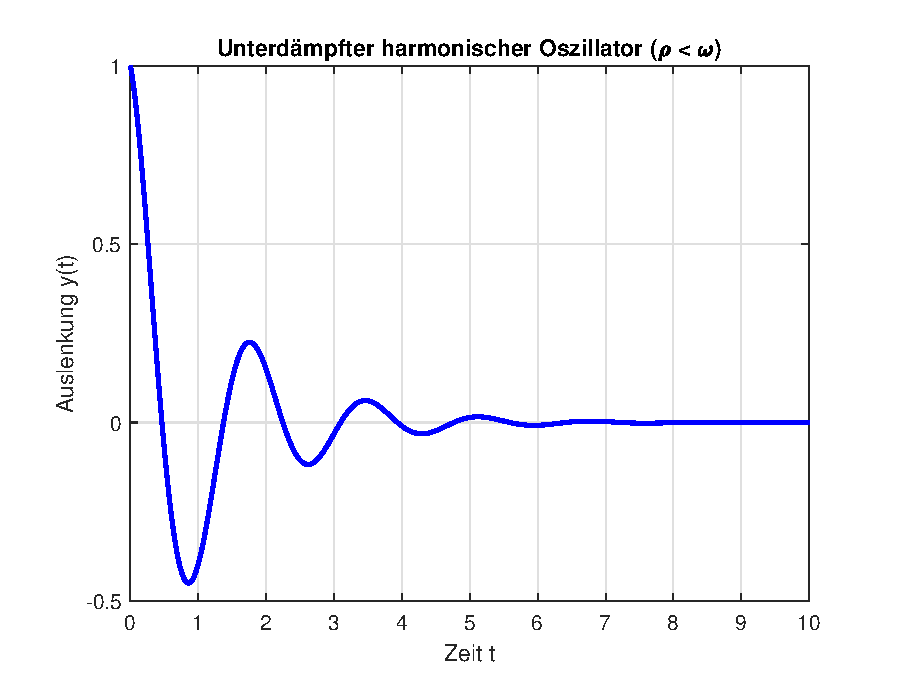
\includegraphics[width=0.3\textwidth]{unterdaempfterHarOszil.eps}
\end{figure}
}

\ErgebnisC{harmonischerOszillatorinhomogen}{
Fall 1: $y(t) = A\operatorname{e}^{(-\rho + \sqrt{\rho^2 - \omega^2})t} + B\operatorname{e}^{(-\rho - \sqrt{\rho^2 - \omega^2})t} + \frac{1}{2\sqrt{\rho^2 -\omega^2}}t \operatorname{e}^{(-\rho +  \sqrt{\rho^2 - \omega^2})t},$\\
Fall 2: $y(t) = (A+Bt) \operatorname{e}^{-\omega t} + \frac{1}{2}t^2 \operatorname{e}^{-\omega t},$\\
Fall 3: $y(t) = \operatorname{e}^{-\rho t}(A \cos(\sqrt{\omega^2 - \rho^2} t) + B \sin(\sqrt{\omega^2 - \rho^2} t))+\frac{1}{2}t\operatorname{e}^{-\rho t} \sin((\sqrt{\omega^2 - \rho^2})t).$
}




% \ifthenelse{\boolean{mitLoes}}{\ruleBig \cleardoublepage}{}
% 
% \Aufgabe[e]{Lineare Differentialgleichungen mit Resonanz}
{
Bestimmen Sie die allgemeine Lösung der folgenden linearen Differentialgleichungen
\begin{abc}
\item $y'' - y = 1$, 
\item $y''' + y'' = 1$, 
\item $y''+y'-2y = e^x$, 
\item $y''+y = \cos(x)$.
\end{abc}
}

\Loesung{
\begin{abc}
\item 
Wir lösen zunächst die homogene Gleichung
$$
y'' -y = 0.
$$
Das charakteristische Polynom ist
$$
\lambda^2 -1 = 0
$$
mit den Nullstellen $\lambda_1 = 1$ und $\lambda_2 = -1$.
Damit ist die homogene Lösung
$$
y_h = c_1 \operatorname{e}^x + c_2 \operatorname{e}^{-x}
$$
Für die partikuläre Lösung wählen wir den Ansatz
$$
y_p = A
$$
Damit ist 
$$
y_p'' = 0
$$
Eingesetzt in die Differentialgleichung erhalten wir
$$
0 - A = 1
$$
Also ist $y_p = -1$.
Die allgemeine Lösung ist dann 
\begin{align*}
y &= y_h + y_p\\
  &= c_1 \operatorname{e}^x + c_2 \operatorname{e}^{-x} -1
\end{align*}
\item
Wir lösen zunächst die homogene Gleichung
$$
y''' + y'' = 1.
$$
Das charakteristische Polynom ist
$$
\lambda^3 + \lambda^2 = \lambda^2(\lambda +1)= 0
$$
mit der doppelten Nullstelle $\lambda = 0$ und der einfachen Nullstelle $\lambda = -1$.
Damit ist die homogene Lösung
$$
y_h = (c_1+c_2x)+ c_3\operatorname{e}^{-x}
$$
Da $\lambda = 0$ eine doppelte Nullstelle ist und die rechte Seite eine Konstante, haben 
wir hier einen Fall mit Resonanz und wählen für die partikuläre Lösung den Ansatz
$$
y_p = Ax^2
$$
Wir bestimmen die Ableitungen
$$
y_p' = 2Ax \, , \, y_p'' = 2A \, , \, y_p''' = 0
$$
und setzen sie in die Differentialgleichung ein.
$$
0 + 2A = 1
$$
Damit ist $A = \frac{1}{2}$ und die partikuläre Lösung
$$
y_p = \frac{x^2}{2}.
$$
Die allgemeine Lösung ist
\begin{align*}
y &= y_h + y_p\\
  &= (c_1+c_2x)+ c_3\operatorname{e}^{-x} +\frac{x^2}{2}.
\end{align*}
\item
Wir lösen zunächst homogene Gleichung
$$
y''+y'-2y = 0.
$$
Das charakteristische Polynom ist
$$
\lambda^2 + \lambda -2 = 0
$$
mit den Nullstellen $\lambda_1 = -2$ und $\lambda_2 = 1$.
Damit ist die homogene Lösung
$$
y_h = c_1 \operatorname{e}^{-2x} + c_2 \operatorname{e}^x
$$
Wir haben hier wieder einen Fall mit Resonanz. Daher wählen wir für die partikuläre 
Lösung den Ansatz
$$
y_p = Ax \operatorname{e}^x
$$
Wir bestimmen die Ableitungen
\begin{align*}
y_p' &= A \operatorname{e}^x + Ax\operatorname{e}^x\\
y_p'' &= 2A \operatorname{e}^x + Ax\operatorname{e}^x
\end{align*}
In die Gleichung eingesetzt erhalten wir 
\begin{align*}
2A \operatorname{e}^x + Ax\operatorname{e}^x + A \operatorname{e}^x + Ax\operatorname{e}^x
 -2Ax \operatorname{e}^x  &= \operatorname{e}^x \\
 3A \operatorname{e}^x &= \operatorname{e}^x
\end{align*}
Wir erhalten dann $A = \frac{1}{3}$.
Die partikuläre Lösung ist dann also
$$
y_p = \frac{x \operatorname{e}^x}{3}
$$
Die allgemeine Lösung ist dann
\begin{align*}
y &= y_h + y_p \\
  &= c_1 \operatorname{e}^{-2x} + c_2 \operatorname{e}^x + \frac{x \operatorname{e}^x}{3}
\end{align*}
\item
Wir lösen zunächst die homogene Gleichung
$$
y'' + y = 0
$$
mit dem charakteristischen Polynom
$$
\lambda^2 + 1 = 0.
$$
Die Nullstellen sind $\lambda = \pm \operatorname{i}$
Damit ist die homogene Lösung
$$
y_h = c_1 \cos(x) + c_2\sin(x) 
$$
Als Ansatz für die partikuläre Gleichung wählen wir 
$$
y_p = x(A \cos(x) + B \sin(x))
$$
Wir erhalten die Ableitungen
\begin{align*}
y_p' &= (A+Bx) \cos(x) + (B-Ax)\sin(x)\\
y_p'' &= (2B-Ax)\cos(x) - (2A+Bx)\sin(x)
\end{align*}
Wir setzen die Ableitungen in die Gleichung ein 
$$
(2B-Ax)\cos(x) - (2A+Bx)\sin(x) + x(A \cos(x) + B \sin(x)) = \cos(x)
$$
Durch Koeffizientenvergleich erhalten wir $A = 0$ und $B = \frac{1}{2}$.
Die partikuläre Lösung ist damit 
$$
y_p = x \frac{1}{2} \sin(x)
$$
Die allgemeine Lösung ist
\begin{align*}
y &= y_h + y_p \\
  &=  c_1 \cos(x) + c_2\sin(x) + x \frac{1}{2} \sin(x)
\end{align*}

\end{abc}
}

% \ifthenelse{\boolean{mitLoes}}{\ruleBig \cleardoublepage}{}
% 
% \Aufgabe[e]{Laplace-Transformierte}
{
Berechnen Sie die Laplace-Transformierte von $f(t)=\sqrt{t}$: 
$$F(s):=\int\limits_0^\infty\EH{-st}\cdot\sqrt{t}\d t.$$
\textbf{ Hinweise}:
\begin{itemize}
\item Substituieren Sie $u=\sqrt t$. 
\item Spalten Sie $u^2$ in $u\cdot u$ auf und integrieren Sie partiell. 
\item Das Quadrat des verbleibenden Integrals k\"onnen Sie l\"osen, indem Sie Polarkoordinaten einführen.
\end{itemize}
}

\Loesung{
Mit der Substitution \ $u=\sqrt{t} \ \Rightarrow \ \text dt=2\,u\,\text du$ \ erhält man
	\[
	F(s) = \int\limits_{0}^{\infty} \EH{-s\,u^2}\cdot u\cdot 2\,u\ \text du = -\dfrac{1}{s}\cdot\int\limits_{0}^\infty  u\cdot(-2s u)\,\EH{-s\,u^2}\ \text du\ .
\]
Die partielle Integration ergibt
	\begin{align*}
	F(s) & = -\dfrac{1}{s}\left(u\EH{-s\,u^2}\Big|_0^\infty - \int\limits_{0}^\infty  
\EH{-s\,u^2}\ \text du\right)\\[1ex]
& =-\dfrac{1}{s}\left(0-0 - \int\limits_{0}^\infty  
\EH{-s\,u^2}\ \text du\right)\\[1ex]
&  = \dfrac{1}{s}\cdot\int\limits_{0}^\infty  \EH{-s\,u^2}\ \text du  \ .
\end{align*}
Mit Quadrieren erhält man
  \[
  \big(F(s)\big)^2 \ = \ \dfrac{1}{s}\,\int\limits_{0}^\infty \EH{-s\,x^2}\ \text dx 
                   \cdot \dfrac{1}{s}\,\int\limits_{0}^\infty \EH{-s\,y^2}\ \text dy \ = \ 
                   \dfrac{1}{s^2}\,\int\limits_{0}^\infty  \int\limits_{0}^\infty  \EH{-s\,(x^2+y^2)}\ \text dx\,\text dy 
\]
und durch Übergang zu Polarkoordinaten
  \[
  \big(F(s)\big)^2 \ = \ \dfrac{1}{s^2}\,\int\limits_{0}^\infty  \int\limits_{0}^{\pi/2} \EH{-s\,r^2}\ r\,\text d\phi\,\text dr \ = \
         \dfrac{1}{s^2}\cdot\dfrac{\pi}{2}\cdot \left[\frac{-1}{2\,s}\,\EH{-s\,r^2}\right]_0^\infty \ = \ \dfrac{\pi}{4\,s^3} \ .
\]
Damit ist 
\[
\ F(s) = {\cal L}\left(\sqrt{t}\right) = \sqrt{\dfrac{\pi}{4\,s^3}}\ .
\]
}



\ErgebnisC{AufglaplacTrafBere001}
{
$F(s)=\sqrt{\frac{\pi}{4s^3}}\,.$
}

% \ifthenelse{\boolean{mitLoes}}{\ruleBig \cleardoublepage}{}
% 
% \Aufgabe[e]{Laplace-Transformierte}
{
\begin{abc}
\item Berechnen Sie die Laplace-Transformierte 
$$\mathcal{L}\{f(t)\}=F(s)=\int\limits_{t=0}^\infty \EH{-st}\cdot f(t)\d t$$ der folgenden Funktionen: 
\begin{iii}
\begin{multicols}{2}
\item $f(t) = 1$,
\item $f(t) = t$,
\item $f(t) = t^2$,
\item $f(t) = t^3$,
\item $f(t) = e^{-at}$,
\item $f(t) = e^{-at}\cdot t$,
\item ${\mathcal L}\{g'(t)\}$, f\"ur eine allgemeine (gegebene) Funktion $g(t)$,
\item ${\mathcal L}\{g''(t)\}$, f\"ur eine allgemeine (gegebene) Funktion $g(t)$.
\end{multicols}
\end{iii}
\textbf{Hinweis}: F\"ur die letzten beiden Aufgaben kann die Laplacetransformierte $G(s)=\sL\{g(t)\}$ der Funktion $g(t)$ als bekannt vorausgesetzt werden. 

\item Berechnen Sie die Laplace-Transformierte von $f(t)=\sqrt{t}$. \\
\end{abc}
\textbf{Hinweise}:
\begin{itemize}
\item Substituieren Sie $u=\sqrt t$. 
\item Spalten Sie $u^2$ in $u\cdot u$ auf und integrieren Sie partiell. 
\item Das Quadrat des verbleibenden Integrals k\"onnen Sie l\"osen, indem Sie Polarkoordinaten einführen.
\end{itemize}
}

\Loesung{
\begin{abc}
\item Diese Laplace-Transformationen müssen durch Anwendung der Definition und Bestimmung der Integrale berechnet werden. Es wird in der Regel partiell integriert. 
\begin{iii}
\item \begin{align*}
\mathcal{L}\{1\} =& \int\limits_{t=0}^\infty \EH{-st}1 \d t
= \left[\frac{\EH{-st}}{-s}\right]_{t=0}^\infty\\
=&  \dfrac{1}{s}
\end{align*}
\item \begin{align*}
\mathcal{L}\{t\} =& \int\limits_{t=0}^\infty \EH{-st}t \d t
= \left[t\frac{\EH{-st}}{-s}\right]_{t=0}^\infty+\frac 1 s\int\limits_{t=0}^\infty \EH{-st}\d t\\
=& 0 - \left.\frac{\EH{-st}}{-s^2}\right|_{t=0}^\infty
= \dfrac{1}{s^2}
\end{align*}
\item \begin{align*}
\mathcal{L}\{t^2\}  =& \int\limits_{t=0}^\infty t^2\EH{-st} \d t
= \left[t^2\frac{\EH{-st}}{-s}\right]_{t=0}^\infty+\frac 1 s \int\limits_{t=0}^\infty 2t\EH{-st}\d t\\
=& 0 + \left[\frac{2t\EH{-st}}{-s^2}\right]_{t=0}^\infty + \frac{2}{s^2}\int\limits_{t=0}^\infty \EH{-st}\d t\\
=&  0 +\left.\frac{2\EH{-st}}{-s^3}\right|_{t=0}^\infty= \dfrac{2}{s^3}
\end{align*}

\item \begin{align*}
\mathcal{L}\{t^3\}  =& \int\limits_{t=0}^\infty t^3\EH{-st} \d t
= \left[t^3\frac{\EH{-st}}{-s}\right]_{t=0}^\infty+\frac 1 s \int\limits_{t=0}^\infty 3t^2\EH{-st}\d t\\
=& 0 + \left[\frac{3t^2\EH{-st}}{-s^2}\right]_{t=0}^\infty + \frac{3}{s^2}\int\limits_{t=0}^\infty 2t\EH{-st}\d t\\
=&  0 +\left.\frac{6t\EH{-st}}{-s^3}\right|_{t=0}^\infty+\int\limits_{t=0}^\infty\frac{6\EH{-st}}{s^3}\d t\\
=& 0 + \left. \frac{6\EH{-st}}{s^4} \right|_{t=0}^\infty = \frac 6{s^4}
\end{align*}

\item \begin{align*}
\mathcal{L}\{\EH{-at}\} =& \int\limits_{t=0}^\infty \EH{-st}\EH{-at} \d t
= \left[\frac{\EH{-(s+a)t}}{-(s+a)}\right]_{t=0}^\infty\\
=&  \dfrac{1}{s+a}
\end{align*}

\item \begin{align*}
\mathcal{L}\{t\EH{-at}\} =& \int\limits_{t=0}^\infty t\EH{-at}\EH{-st} \d t
= \left[\frac{t\EH{-(s+a)t}}{-(s+a)}\right]_{t=0}^\infty+\frac 1{s+a}\int\limits_{t=0}^\infty \EH{-(s+a)t}\d t \\
=& 0 + \left.\frac{\EH{-(s+a)t}}{-(s+a)^2}\right|_{t=0}^\infty
=  \dfrac{1}{(s+a)^2}
\end{align*}

\item \begin{align*}
\mathcal{L}\{g'(t)\} =& \int\limits_{t=0}^\infty \EH{-st}g'(t) \d t\\
=& \left[\EH{-st}g(t)\right]_{t=0}^\infty - \int\limits_{t=0}^\infty(-s\EH{-st}g(t))\d t\\
=& 0-g(0)+s\mathcal{L}\{g(t)\}
= sG(s)-g(0)
\end{align*}

\item \begin{align*}
\mathcal{L}\{g''(t)\} =& \int\limits_{t=0}^\infty \EH{-st}g''(t) \d t\\
=&\left[\EH{-st}g'(t)\right]_{t=0}^\infty - \int\limits_{t=0}^\infty(-s\EH{-st}g'(t))\d t\\
=& 0-g'(0)+s\mathcal{L}\{g'(t)\}\\
=& s(sG(s)-g(0))-g'(0) = s^2G(s)-g'(0)-sg(0)
\end{align*}

\end{iii}

\item Mit der Substitution \ $u=\sqrt{t} \ \Rightarrow \ \text dt=2\,u\,\text du$ \ erhält man
	\[
	F(s) = \int\limits_{0}^{\infty} \EH{-s\,u^2}\cdot u\cdot 2\,u\ \text du = -\dfrac{1}{s}\cdot\int\limits_{0}^\infty  u\cdot(-2s u)\,\EH{-s\,u^2}\ \text du\ .
\]

Partielle Integration ergibt
	\begin{align*}
	F(s) & = -\dfrac{1}{s}\left(u\EH{-s\,u^2}\Big|_0^\infty - \int\limits_{0}^\infty  
\EH{-s\,u^2}\ \text du\right)\\[1ex]
& =-\dfrac{1}{s}\left(0-0 - \int\limits_{0}^\infty  
\EH{-s\,u^2}\ \text du\right)\\[1ex]
&  = \dfrac{1}{s}\cdot\int\limits_{0}^\infty  \EH{-s\,u^2}\ \text du  \ .
\end{align*}

Durch Quadrieren der Gleichung  erh\"alt man
  \[
  \big(F(s)\big)^2 \ = \ \dfrac{1}{s}\,\int\limits_{0}^\infty \EH{-s\,x^2}\ \text dx 
                   \cdot \dfrac{1}{s}\,\int\limits_{0}^\infty \EH{-s\,y^2}\ \text dy \ = \ 
                   \dfrac{1}{s^2}\,\int\limits_{0}^\infty  \int\limits_{0}^\infty  \EH{-s\,(x^2+y^2)}\ \text dx\,\text dy 
\]
und durch Übergang zu Polarkoordinaten
  \[
  \big(F(s)\big)^2 \ = \ \dfrac{1}{s^2}\,\int\limits_{0}^\infty  \int\limits_{0}^{\pi/2} \EH{-s\,r^2}\ r\,\text d\phi\,\text dr \ = \
         \dfrac{1}{s^2}\cdot\dfrac{\pi}{2}\cdot \left[\frac{-1}{2\,s}\,\EH{-s\,r^2}\right]_0^\infty \ = \ \dfrac{\pi}{4\,s^3} \ .
\]
Damit ist 
	\[
	 F(s) = {\cal L}\left(\sqrt{t}\right) = \sqrt{\dfrac{\pi}{4\,s^3}} .
\]
\end{abc}
}



\ErgebnisC{AufglaplacTrafBere01b}
{
\textbf{a)}\begin{multicols}{3}
\begin{iii}
\item $\dfrac{1}{s}$,
\item $\dfrac{1}{s^2}$,
\item $\dfrac{2}{s^3}$,
\item $\dfrac{3!}{t^4}$,
\item $\frac{1}{s+a}$,
\item $\dfrac{1}{(s+a)^2}$,
\item $ sG(s) - g(0)$,
\item $ s^2G(s) - sg(0) - g'(0)$.
\end{iii}
\end{multicols}
\textbf{b)}$F(s)=\sqrt{\frac{\pi}{4s^3}}\,.$
}

% \ifthenelse{\boolean{mitLoes}}{\ruleBig \cleardoublepage}{}
% 
\Aufgabe[e]{Anfangswertprobleme zu linearen Differentialgleichungen $n$-ter Ordnung}
{
Gegeben seien die folgenden Anfangswertprobleme: 
\begin{abc}
\item $y^{\prime\prime}(t) - 2 y^\prime(t) - 3y(t) = 4 \EH{t}, \quad y(0) = 0, 
         \quad y'(0) = 6,$
\item $y^{\prime\prime}(t)+4y^\prime(t)+4y(t)=4 \EH{-2t}, \quad y(0)=1 ,\quad
  y^\prime(0)=0$.
\end{abc}
Bestimmen Sie die L\"osungen jeweils mit Hilfe des Exponentialansatzes \textbf{und} zus\"atzlich mit Hilfe der Laplace-Transformation. 
}

\Loesung{
Zun\"achst die L\"osung mittels Exponentialansatz: \\
\begin{abc}
\item Die Nullstellen des charakteristischen Polynoms
$p(\lambda)=\lambda^2-2\lambda-3$ sind $\lambda_1=-1$ und $\lambda_2=3$. 
Eine Partikul\"arl\"osung der inhomogenen Gleichung berechnet man mit
dem Ansatz $y_p(t)=ae^t$, es folgt
$ -4 a e^t \stackrel{!}{=}4e^t$ und damit $a=-1$. Die allgemeine L\"osung
ist 
$$ y_{allg}(t) = - e^t + c_1 \EH{-t} + c_2 \EH{3t} \ \text{ mit } c_1,c_2 \in \R .$$
Aus den Anfangsbedingungen $y(0)=-1+c_1+c_2 \stackrel{!}{=} 0$
und $y^\prime(0) = -1 - c_1 + 3c_2 \stackrel{!}{=} 6$ folgt das lineare 
Gleichungssystem
$$ \begin{array}{rcrl}
   c_1 & + & c_2 & = 1, \\
   -c_1 & + & 3c_2 & = 7 
   \end{array} $$
mit L\"osung $c_2=2$ und $c_1=-1$. Damit ist 
$$ y_{AWP}(t) = -e^t-\EH{-t}+2\EH{3t}. $$

\item Die Nullstelle von $p(\lambda)=\lambda^2+4\lambda+4$ ist
$\lambda=-2$, dies ist eine doppelte Nullstelle. Als Ansatz f\"ur die
Partikul\"arl\"osung muss man 
$y_p(t)=at^2 \EH{-2t}$ nehmen, denn man hat Resonanz der Ordnung 2. 
Mit $y_p^\prime(t) = a \EH{-2t} \big( 2t-2t^2\big)$
und $y_p^{\prime\prime}(t) = a \EH{-2t} \big(2-8t+4t^2\big)$
folgt
$2a \EH{-2t} \stackrel{!}{=} 4 \EH{-2t}$ und damit $a=2$. 
Dies liefert die allgemeine L\"osung
$$ y_{allg}(t) = \big( 2t^2 + c_1 t + c_2 \big) \EH{-2t}
   \ \text{ mit } c_1,c_2 \in \R. $$
Die Anfangsbedingungen  $y(0)=c_2 \stackrel{!}{=} 1$ und
$y^\prime(0) = c_1-2c_2 \stackrel{!}{=} 0$ liefern $c_2=1$ und $c_1=2$ 
und damit die L\"osung
$$ y_{AWP}(t) = \big( 2t^2 + 2t + 1 \big) \EH{-2t} . $$ 
\end{abc}
Nun die L\"osung mit Hilfe der Laplace-Transformation: 
\begin{abc}
\item Die Laplace-Transformation der Differentialgleichung ergibt
\begin{align*}
&&\sL\{4\EH{t}\}=&\sL\{y''(t)-2y'(t)-3y(t)\}\\
\Rightarrow&&\frac{4}{s-1}=&s^2Y(s)-y'(0)-sy(0)-2(sY(s)-y(0))-3Y(s)\\
&&=&s^2Y(s)-6-2sY(s)-3Y(s)
\end{align*}
Die L\"osung im Bildbereich ist dann
\begin{align*}
Y(s)=&\frac 1{s^2-2s-3}\cdot \left( \frac 4{s-1}+6\right)\\
=& \frac{6s-2}{(s-1)(s-3)(s+1)}
\end{align*}
Diese l\"asst sich mittels Partialbruchzerlegung darstellen als 
\begin{align*}
Y(s)=& \frac{-1}{s-1} + \frac{2}{s-3} + \frac{-1}{s+1}
\end{align*}
und die R\"ucktransformation ergibt die L\"osung des Anfangswertproblems: 
\begin{align*}
y(t)=& -\sL^{-1}\left\{\frac{1}{s-1}\right\} + 2 \sL^{-1}\left\{\frac 1{s-3}\right\} -\sL^{-1}\left\{\frac 1{s+1}\right\}\\
=& - \EH{t} + 2 \EH{3t}-\EH{-t}
\end{align*}
\item Die Laplace-Transformation der Differentialgleichung ergibt
\begin{align*}
&&\sL\{4\EH{-2t}\}=&\sL\{y''(t)+4y'(t)+4y(t)\}\\
\Rightarrow&&\frac{4}{s+2}=&s^2Y(s)-y'(0)-sy(0)+4(sY(s)-y(0))+4Y(s)\\
&&=&s^2Y(s)-s+4sY(s)-4+4Y(s)
\end{align*}
Die L\"osung im Bildbereich ist dann
\begin{align*}
Y(s)=&\frac 1{s^2+4s+4}\cdot \left( \frac 4{s+2}+s+4\right)\\
=& \frac{s^2+6s+12}{(s+2)^3}
\end{align*}
Diese l\"asst sich mittels Partialbruchzerlegung darstellen als 
\begin{align*}
Y(s)=& \frac{1}{s+2} + \frac{2}{(s+2)^2} + \frac{4}{(s+2)^3}
\end{align*}
und die R\"ucktransformation ergibt die L\"osung des Anfangswertproblems: 
\begin{align*}
y(t)=& \EH{-2t}+2t\EH{-2t}+4\frac{t^2\EH{-2t}}{2}
= \EH{-2t}(1+2t+2t^2)
\end{align*}
\end{abc}
 
}


\ErgebnisC{gewdglLineAWPr001}
{
a) $y(t) = -e^t-\EH{-t}+2\EH{3t}$\\
b) $y(t) = \big( 2t^2 + 2t + 1 \big) \EH{-2t}$
}

\ifthenelse{\boolean{mitLoes}}{\ruleBig \cleardoublepage}{}

% \Aufgabe[e]{$\delta$--Distribution}
{
Bestimmen Sie die folgenden Integrale:
\begin{iii}
\item $ I_1 = \int\limits_{-\infty}^{\infty} \dfrac{\cos(x)}{1+x^2} \cdot \delta(x - \pi) \, \text{d}x $ \\
\item $ I_2 = \int\limits_{-\pi/2}^{\pi/2} \cos(x) \cdot \delta(x - \pi) \, \text{d}x $\\
\item $ I_3 = \int\limits_{-1}^5 \dfrac{e^{x^2 + 3}}{x + 2} \cdot \delta(x) \, \text{d}x $\\
\item $I_4 = \int\limits_{-1}^{1} (f(x) - f(0)) \cdot \delta\left(x + \frac{1}{2} \right) \, \text{d}x$
\end{iii}
}
\Loesung{
\begin{iii}
\item 
$$
 I_1=\int\limits_{-\infty }^{\infty} \dfrac{\cos (x)}{1+x^2}\cdot \delta \left( x-\pi \right) \;\text{d}x 
                      = \dfrac{\cos (\pi)}{1+\pi^2} = \dfrac{-1}{1+\pi^2}\ .\\
$$                      
\item
$$
 I_2=\int\limits_{-\pi /2}^{\pi /2}\cos (x)\cdot \delta \left( x-\pi \right) \;\text{d}x = 0 \quad \text{da}\quad 
                     \pi\notin[-\pi/2\,,\,\pi/2]\ .
$$
\item
$$
I_3 = \int\limits_{-1}^5 \dfrac{e^{x^2 + 3}}{x + 2} \cdot \delta(x) \, \text{d}x  = \dfrac{e^{0^2+3}}{0+2} = \dfrac{e^3}{2} \ .
$$

\item
$$
I_4 = \int\limits_{-1}^{1} (f(x) - f(0)) \cdot \delta\left(x + \frac{1}{2} \right) \, \text{d}x = f(-1/2)-f(0)\ .
$$
\end{iii}
}




\ErgebnisC{laplacDeltDist002}{
\begin{iii}
\item $I_1 =\dfrac{-1}{1+\pi^2}$
\item $I_2 =0$
\item $I_3 = \dfrac{e^{0^2+3}}{0+2} = \dfrac{e^3}{2}$
\item $I_4 =f(-1/2)-f(0) $
\end{iii}
}

% \ifthenelse{\boolean{mitLoes}}{\ruleBig \cleardoublepage}{}

\Aufgabe[e]{Laplace--Transformierte}
{
Bestimmen Sie unter Verwendung von \ ${\cal{L}}\big\{\sin(t)\big\} = \dfrac{1}{s^2+1}$ \ und geeigneten Rechenregeln folgende Ausdr\"ucke
	\[
	\textbf{a)} \ {\cal{L}}\left\{\frac{\sin(t)}{t}\right\}\ ,\quad
	\textbf{b)} \ {\cal{L}}\left\{\int\limits_0^t\frac{\sin(\tau)}{\tau}\ \text d\tau\right\}\ ,\quad
	\textbf{c)} \ \int\limits_{0}^{\infty}\frac{\sin(t)}{t}\ \text dt\ ,\quad
	\textbf{d)} \ {\cal{L}}\left\{\EH{-t}\,\frac{\sin(t)}{t}\right\}\ .
\]



\textbf{e)} \ Bestimmen Sie \textbf{mit Hilfe des Faltungssatzes} der Laplace-Transformation die Urbildfunktion \  $f(t)$ \ zur Bildfunktion
  \[
  F(s) := \dfrac{s}{(s+1)(s^2+1)}\ .
\]
}

\Loesung{
\textbf{a)} \ Mit der Transformationsformel \ \ ${\cal{L}}\left\{\dfrac{f(t)}{t}\right\} = \int\limits_{s}^\infty  F(\sigma)\ \text d\sigma$ \ \ erhält man
	\[
	{\cal{L}}\left\{\frac{\sin(t)}{t}\right\} = \int\limits_{s}^\infty  \dfrac{1}{\sigma^2+1}\ \text d\sigma = \Big[\arctan(\sigma)\Big]_s^\infty = \dfrac \pi2-\arctan(s)\ .
\]

\textbf{b)} \ Mit der Transformationsformel \ \ ${\cal{L}}\left\{\int\limits_{0}^{t} f(\tau) \text d\tau\right\} = \dfrac{F(s)}{s}$ \ \ erhält man 
	\[
	{\cal{L}}\left\{\int\limits_{0}^{t}\frac{\sin(\tau)}{\tau}\ \text d\tau\right\} = \frac 1s\cdot\left(\dfrac \pi2-\arctan(s) \right)
\]


\textbf{c)}

\textbf{1. Lösungsweg}\newline
Mit Hilfe des Anfangs- und Endwertsatzes ergibt sich 
\begin{align*}
\int\limits_{0}^\infty\frac{\sin(t)}{t}\ \text dt
	   =& \lim_{t\to\infty} \int\limits_{0}^t\frac{\sin\tau}{\tau}\d \tau = \lim_{s\to 0}\left(
	   s\cdot {\cal{L}}\left\{\int\limits_{0}^t\frac{\sin(\tau)}{\tau}\d \tau\right\}\right) \\
=& \lim_{s\to 0}\left(\dfrac \pi2-\arctan(s) \right) = \dfrac \pi2\ .
\end{align*}

\textbf{2. Lösungsweg}\newline
Nach Definition der Laplace-Transformierten gilt
$${\cal{L}}\left\{\dfrac{\sin(t)}{t}\right\}=\int\limits_{0}^\infty\EH{-st}\cdot\frac{\sin(t)}{t}\ \text dt=U(s)$$

Aus der Teilaufgabe \textbf{a)} folgt $U(s)=\dfrac \pi2-\arctan(s)$.\newline
Somit erhält man
$$\int\limits_{0}^\infty\frac{\sin(t)}{t}\ \text dt=\int\limits_{0}^\infty\EH{-0\cdot t}\cdot\frac{\sin(t)}{t}\ \text dt=U(0)=\dfrac \pi2$$





\textbf{d)} \ Mit der Transformationsformel \ \ ${\cal{L}}\left\{\EH{-at}\,f(t)\right\} = F(s+a)$ \ \ erhält man
	\[
	{\cal{L}}\left\{\EH{-t}\,\frac{\sin(t)}{t}\right\} = \dfrac \pi2-\arctan(s+1)\ .
\]


\textbf{e)} \ Es gilt
$$
F(s) = F_1(s) \cdot F_2(s) \quad \mbox{mit} \quad F_1(s) = \dfrac{1}{s+1}\,, \quad F_2(s)= \dfrac{s}{s^2+1}\,.
$$
Mit den Rücktransformierten 
$$
f_1(t) = \EH{-t} \quad \mbox{und} \quad f_2(t) = \cos( t)
$$
folgt
\begin{align*}
f(t) & = f_1(t) \ast f_2(t) = \int_0^t \EH{-(t-\tau)}\cos (\tau) \text d \tau = \EH{-t} \int_0^t \EH{\tau}\cos (\tau) \text d \tau\,.
\end{align*}
Mit 
\begin{align*}
I=&\int_0^t \EH{\tau}\cos \tau \text d \tau  = \EH{\tau}\sin \tau\Big|_0^t -  \int_0^t \EH{\tau}\sin \tau \text d \tau\\[1ex]
& =  \EH{t}\sin t + \EH{\tau}\cos \tau |_0^t - \int_0^t \EH{\tau}\cos \tau \text d \tau\\[1ex]
& =  \EH{t}\sin t + \EH{t}\cos t - 1  - I
\end{align*}
folgt
$$2I=\EH{t}\sin t + \EH{t}\cos t - 1$$
und
$$
I = \dfrac{1}{2}\,\EH{t}\sin t + \dfrac{1}{2}\,\EH{t}\cos t - \dfrac{1}{2}
$$


Alternativ kann man im Komplexen rechnen:
\begin{align*}
I=&\int_0^t \EH{\tau}\cos \tau \text d \tau  =\int_0^t \Real(\EH{\tau}\cdot\EH{i\tau})  \text d \tau \\[1ex]
&=\Real\left(\int_0^t (\EH{(1+i)\tau}\text d \tau\right) =\left[\Real\left(\dfrac{\EH{(1+i)\tau}}{1+i}\right)\right]_0^t=\left[\EH{\tau}\Real\left(\dfrac{(\cos\tau+i\sin\tau)(1-i)}{2}\right)\right]_0^t\\[1ex]
&=\left[\EH{\tau}\cdot\dfrac{(\cos\tau+\sin\tau)}{2}\right]_0^t=\EH{t}\cdot\dfrac{(\cos t+\sin t)}{2}-\dfrac{1}{2}\\
\end{align*}

Somit ergibt sich
$$
\ f(t) = \EH{-t} \cdot I=\dfrac{1}{2} (\sin t + \cos t) - \dfrac{1}{2}\,\EH{-t}\ .\ 
$$

}

\ErgebnisC{AufglaplacTrafBere002}
{
\textbf{ a)} $\frac \pi 2 - \arctan s$, 
\textbf{ b)} $\frac {\pi/2-\arctan s} s$, 
\textbf{ c)} $\frac \pi 2$,
\textbf{ d)} $\frac \pi 2 - \arctan (s+1)$,
\textbf{ e)} $\frac {\sin t + \cos t}2 - \frac{\EH{-t}}2$
}

\ifthenelse{\boolean{mitLoes}}{\ruleBig \cleardoublepage}{}

% \Aufgabe[e]{Lineare Differentialgleichung}
% {
% Gegeben sei das Anfangswertproblem für \ $u(t)$
% $$	u'' + 4\,u' +3\,u = 12\cdot\Big(1-h(t-2)\Big)\ ,\quad u(0)=u'(0)=0$$
% wobei \ $h(t)$ \ die Heaviside--Funktion ist.


% \textbf{a)} \ Bestimmen Sie die Lösung mit Hilfe der Laplace--Transformation.

% \textbf{b)} \ Geben Sie die Lösung in den Bereichen  $0\le t < 2$  und  $ 2\le t$ ohne Verwendung der Heaviside--Funktion an und fassen Sie die Terme sinnvoll zusammen.

% }
\Aufgabe[e]{Linear ODE}
{
Gegeben sie das folgende Anfangswertproblem für $y(t)$ durch
$$	y'' + 4\,y = t\ ,\quad y(0)= 1, y'(0)=2.$$

\textbf{a)} \ Berechnen Sie die Lösung mit dem Exponentialansatz.

\textbf{b)} \ Berechnen Sie die Lösung mit Hilfe der Laplace-Transformation.

}

\Loesung{
\textbf{a)} 
Die allgemeine Lösung ist gegeben durch die Lösung des homogenenen Systems und der 
partikulären Lösung
% The solution is given by the solution of the homogeneous system plus a particular solution
$$y(t) = y_h(t) + y_p(t).$$
Für das homogene System betrachten wir die Nullstellen des charakteristischen Polynoms
% For the homogeneous system we consider the zeros of the characteristic polynomial
$$\lambda^2+4=0,$$
welche die komplex Konjugierten sind
% which are the complex conjugates
$$\lambda = \pm 2\operatorname{i}.$$
Daher ist die Lösung des homogenen Systems
% Therefore, the solution of the homogeneous system is
$$y_h(t) = C_1 \cos{2t} + C_2 \sin{2t}.$$
Die beiden Konstanten werden mit den Anfangswerten bestimmt.
% The two constants will be determined with the initial conditions.

Für die partikuläre Lösung machen wir den Ansatz
% For the particular solution we make the ansatz
$$y_p(t) = A_0 + A_1 t,$$
weil die rechte Seite der Differentialgleichung ein lineares Polynom ist.
% because the right hand side of the differential equation is a linear polynomial.
Die beiden Konstanten $A_0$ und $A_1$ werden durch einsetzen in deiGleichung bestimmt.
% The two constants $A_0$ and $A_1$ are determined inserting the solution in the equation.
Da $y'=A_1$ und $y''=0$, erhalten wir
$$4(A_0+A_1t) = t$$
und mit Koeffizientenvergleich gilt
% and the coefficients comparison gives 
$$A_0=0, \qquad A_1 = \frac{1}{4}.$$
Insgesamt ergibt sich die allgemeine Lösung
$$y(t) = \frac{1}{4}t + C_1 \cos{2t} + C_2 \sin{2t}.$$
Aus den Anfangswerten erhalten wir
$$y(0) = C_1 = 1$$
und 
$$y'(0)= \frac{1}{4} + 2C_2 \stackrel{!}{=} 2 \rightarrow C_2 = \frac{7}{8}.$$
Die spezielle Lösung ist dann
% The solution is
$$y(t) = \frac{1}{4}t+\cos{2t} + \frac{7}{8}\sin{2t}.$$

\textbf{b)}
Mit der Laplace-Transformation gilt
% With the Laplace transform it is
$$s^2Y(s) -s-2+4Y(s) = \frac{1}{s^2}$$
$$(s^2+4)Y(s) = \frac{1}{s^2}+s+2$$
$$Y(s) = \frac{s^3+2s^2+1}{s^2(s^2+4)}$$
Partialbruchzerlegung
$$\frac{s^3+2s^2+1}{s^2(s^2+4)}= \frac{A}{s}+ \frac{B}{s^2} + \frac{Cs+D}{s^2+4}$$
Multiplikation beider Seiten mit $s^2(s^2+4)$ 
$$s^3+2s^2+1= As(s^2+4)+ B(s^2+4) + (Cs+D)s^2$$
der Wert $s=0$ führt zu $B=\frac{1}{4}$.
$$s^3+2s^2+1= As^3+4As+ \frac{1}{4}s^2+1 + Cs^3+Ds^2$$
Mit Koeffizientenvergleich erhalten wir
\begin{align*}
A&=0\\
C&=1\\
D+\frac{1}{4}&=2 \quad \rightarrow \quad D=\frac{7}{4}
\end{align*}
$$Y(s) = \frac{1}{4}\cL^{-1}\left\{ \frac{1}{s^2} \right\} + \cL^{-1}\left\{ \frac{s}{s^2+2^2} \right\} + \frac{7}{4}\frac{1}{2}\cL^{-1}\left\{ \frac{2}{s^2+2^2} \right\}$$
$$y(t) = \frac{1}{4}t + \cos{2t} + \frac{7}{8}\sin{2t}.$$

}

%\newcounter{AufglaplacldglKlLp001}
%\setcounter{AufglaplacldglKlLp001}{\theAufg}
%\Ergebnis{\subsubsection*{Ergebnisse zu Aufgabe \arabic{Blatt}.\arabic{AufglaplacldglKlLp001}:}
%
%}

\ifthenelse{\boolean{mitLoes}}{\ruleBig \cleardoublepage}{}

% \Aufgabe[f]{R\"ucktransformation}
% {
% Berechnen Sie
% \begin{align*}
% &\text{\bf a)}&&\, &\mathcal{L}^{-1}\left\{ \frac 5{s+2}\right\}&
% \qquad\qquad\text{\bf b)}& \, &\mathcal{L}^{-1}\left\{\frac {4s-3}{s^2+4}\right\}\\
% &\text{\bf c)}&&\, &\mathcal{L}^{-1}\left\{ \frac {2s-5}{s^2}\right\}&
% \qquad\qquad\text{\bf d)}& \, &\mathcal{L}^{-1}\left\{ \frac 1{s^2+2s}\right\}\\
% &\text{\bf e)}&&\, &\mathcal{L}^{-1}\left\{\frac {5s^2-15s+7}{(s+1)(s-2)^2}\right\}&
% \qquad\qquad\text{\bf f)}&\, &\mathcal{L}^{-1}\left\{\frac {4-5s}{s^{3/2}}\right\}.
% \end{align*}
% }
\Aufgabe[e]{Inverse Laplace-Transformation}
{
Bestimmen Sie
\begin{align*}
&\text{\textbf a)}&&\, &\mathcal{L}^{-1}\left\{ \frac 5{s+2}\right\}&
\qquad\qquad\text{\textbf b)}& \, &\mathcal{L}^{-1}\left\{\frac {4s-3}{s^2+4}\right\}\\
&\text{\textbf c)}&&\, &\mathcal{L}^{-1}\left\{ \frac {2s-5}{s^2}\right\}&
\qquad\qquad\text{\textbf d)}& \, &\mathcal{L}^{-1}\left\{ \frac 1{s^2+2s}\right\}\\
&\text{\textbf e)}&&\, &\mathcal{L}^{-1}\left\{\frac {5s^2-15s+7}{(s+1)(s-2)^2}\right\}&
\qquad\qquad\text{\textbf f)}&\, &\mathcal{L}^{-1}\left\{3\operatorname{e}^{-2s}\right\}\\
&\text{\textbf g)}&&\, &\mathcal{L}^{-1}\left\{ \frac{s}{(s+2)^2+9}\right\}&.
\end{align*}
}
\Loesung{
\begin{abc}
\item $$\mathcal{L}^{-1}\left\{ \dfrac 5 {s+2}\right\} = 5\mathcal{L}^{-1}\left\{\dfrac 1{s+2}\right\} = 5\operatorname{e}^{-2t}$$
\item \begin{align*}
\mathcal{L}^{-1}\left\{ \frac{4s-3}{s^2+4}\right\} 
=&  4 \mathcal{L}^{-1}\left\{\frac
s{s^2+2^2}\right\} - 3 \mathcal{L}^{-1}\left\{\frac 1 {s^2 + 2^2}\right\}\\
=& 4 \cos(2t)-\frac 32 \sin(2t)
\end{align*}
\item $$\mathcal{L}^{-1}\left\{\frac {2s-5}{s^2}\right\}
=2\mathcal{L}^{-1}\left\{\frac 1s\right\} - 5 \mathcal{L}^{-1}\left\{ \frac 1{s^2}\right\} 
= 2 - 5t$$
\item \begin{align*}
\mathcal{L}^{-1}\left\{ \frac 1{s^2+2s}\right\} = &\mathcal{L}^{-1}\left\{ \dfrac {\frac 12}s+ \dfrac {- \frac
12}{s+2}\right\}= \frac 12 \mathcal{L}^{-1}\left\{ \frac 1s\right\}- \frac
12 \mathcal{L}^{-1}\left\{ \frac 1{s+2}\right\}\\
=& \frac 12 - \frac 12 \operatorname{e}^{-2t}
\end{align*}
\item \begin{align*}
\mathcal{L}^{-1}\left\{\frac{5s^2-15s+7}{(s+1)(s-2)^2}\right\} = & 3 \mathcal{L}^{-1}\left\{ \frac 1 {s+1}\right\} +
2 \mathcal{L}^{-1}\left\{ \frac 1 {s-2}\right\} - \mathcal{L}^{-1}\left\{ \frac 1 {(s-2)^2}\right\}\\
=& 3\operatorname{e}^{-t} +2\operatorname{e}^{2t} - t\operatorname{e}^{2t}
\end{align*}
\item 
\begin{align*}
\mathcal{L}^{-1}\left\{3e^{-2s}\right\}=3\delta(t-2)
\end{align*}
\item
\begin{align*}
\mathcal{L}^{-1}\left\{ \frac{s}{(s+2)^2+9}\right\} 
&= \mathcal{L}^{-1}\left\{ \frac{s+2-2}{(s+2)^2+9}\right\} \\
&= \mathcal{L}^{-1}\left\{ \frac{s+2}{(s+2)^2+3^2}\right\}-2 \mathcal{L}^{-1}\left\{ \frac{1}{(s+2)^2+3^2}\right\} \\
&= e^{-2t} \cos(3t) - \frac{2}{3} e^{-2t} \sin(3t)
\end{align*}

%\begin{align*}
%\mathcal{L}^{-1}\left\{\frac{4-5s}{s^{3/2}}\right\}=&4\mathcal{L}^{-1}\left\{\frac{1}{s^{3/2}}\right\}-5 \mathcal{L}^{-1}\left\{\frac{1}{s^{1/2}}\right\}
%=4\mathcal{L}^{-1}\left\{\dfrac{\frac 1{\sqrt s}}{s}\right\} -5 \mathcal{L}^{-1}\left\{\frac{1}{\sqrt s}\right\}\\
%=&4\int_0^t\mathcal{L}^{-1}\left\{\frac{1}{\sqrt s}\right\}\text d t-5\dfrac1{\sqrt{\pi t}}
%=4\int_0^t\dfrac1{\sqrt{\pi t}}\text d t-5\dfrac1{\sqrt{\pi t}}\\
%=&\frac{4}{\sqrt{\pi}}\int_0^t t^{-\frac12}\text d t-5\dfrac1{\sqrt{\pi t}}
%= \frac{8\sqrt t }{\sqrt \pi} - \frac{5}{\sqrt{\pi t}}
%\end{align*}
%
%
%% Alternativ kann man die Formel
%% $$\mathcal{L}^{-1}\left\{\frac{1}{s^{a}}\right\}=\dfrac{t^{a-1}}{\Gamma(a)}$$
%% mit $\Gamma(\frac 12) = \sqrt \pi $ und $\Gamma(\frac 32)=\frac{\sqrt \pi}2$ benutzen.
%Alternatively, the formula
%$$\mathcal{L}^{-1}\left\{\frac{1}{s^{a}}\right\}=\dfrac{t^{a-1}}{\Gamma(a)}$$
%with $\Gamma(\frac 12) = \sqrt \pi $ and $\Gamma(\frac 32)=\frac{\sqrt \pi}2$ can be used.
\end{abc}
}



\ErgebnisC{AufglaplacTrafBere004}
{
{\textbf a)} $5\operatorname{e}^{-2t}                                             $
{\textbf b)} $4 \cos(2t)-\frac 32 \sin(2t)                          $
{\textbf c)} $ 2 - 5t                                               $
{\textbf d)} $\frac 12 - \frac 12 \operatorname{e}^{-2t}                          $
{\textbf e)} $3\operatorname{e}^{-t} +2\operatorname{e}^{2t} - t\operatorname{e}^{2t}                         $
{\textbf f)} $\frac{8\sqrt t }{\sqrt \pi} - \frac{5}{\sqrt{\pi t}}  $

}









\ifthenelse{\boolean{mitLoes}}{\ruleBig \cleardoublepage}{}

% \Aufgabe[f]{AWP mit Laplace--Transformation}
% {
% Bestimmen Sie mit Hilfe der Laplace--Transformation die Lösung der Anfangswertaufgabe: 
% $$ u''(t)+4\,u'(t)-12\,u(t)=4\,\text{e}^{-2\,t}$$
% mit den Anfangswerten 
% $$u(0)=0 \text{ und }  u'(0)=0\;.$$
% %&  &  &  &  &  &  \\ 
% %\mathbf{ii)} &  & v''(t)+25\,v(t)=80\,\sin (3\,t) & , & v(0)=3
% %& , & v'(0)=5\;. \\ 
% %&  &  &  &  &  &  \\ 
% %\mathbf{iii)} &  & w''(t)+25\,w(t)=50\,\sin (5\,t) & , & 
% %w(0)=1 & , & w'(0)=5\;. \\ 
% %&  &  &  &  &  &  \\ 
% %\mathbf{iv)} &  & x''(t)+4\,x'(t)+13\,x(t)=0 & , & 
% %x(0)=6 & , & x'(0)=0\;.

% }
\Aufgabe[e]{IVP with Laplace transform}
{
Compute the solution of the following initial value problem using the Laplace transform:
$$ u''(t)+4\,u'(t)-12\,u(t)=4\,\text{e}^{-2\,t}$$
with the initial values
$$u(0)=0 \text{ and }  u'(0)=0\;.$$
%&  &  &  &  &  &  \\ 
%\mathbf{ii)} &  & v''(t)+25\,v(t)=80\,\sin (3\,t) & , & v(0)=3
%& , & v'(0)=5\;. \\ 
%&  &  &  &  &  &  \\ 
%\mathbf{iii)} &  & w''(t)+25\,w(t)=50\,\sin (5\,t) & , & 
%w(0)=1 & , & w'(0)=5\;. \\ 
%&  &  &  &  &  &  \\ 
%\mathbf{iv)} &  & x''(t)+4\,x'(t)+13\,x(t)=0 & , & 
%x(0)=6 & , & x'(0)=0\;.

}
\Loesung{
%\textbf{i)\ \ }
% Die Laplace--Transformation der AWA lautet mit\ \ $%
% u_{0}=u_{0}'=0$\ : 
% \begin{align*}
% &  & \left( s^{2}\,U(s)-s\,u_{0}-u_{0}'\right) +4\cdot \left(
% s\,U(s)-u_{0}\right) -12\cdot U(s)\;=\;\dfrac{4}{s+2} \\ 
% &  &  \\ 
% \Rightarrow &  & \left( s^{2}+4\,s-12\right) \cdot U(s)\;=\;\dfrac{4}{s+2}
% \\ 
% &  &  \\ 
% \Rightarrow &  & U(s)\;=\;\dfrac{4}{\left( s+2\right) \,\left(
% s^{2}+4\,s-12\right) }\;=\;\dfrac{\frac{-1}{4}}{s+2}+\dfrac{\frac{1}{8}}{s-2}%
% +\dfrac{\frac{1}{8}}{s+6}
% \end{align*}
% Die Rücktransformation ergibt die Lösung der AWA\thinspace : 
% \[
% u_{\text{AW}}(t)=\dfrac{-1}{4}\,\text{e}^{-2\,t}+\dfrac{1}{8}\,\text{e}%
% ^{2\,t}+\dfrac{1}{8}\,\text{e}^{-6\,t}\;\;. 
% \]
With $%
u_{0}=u_{0}'=0$, the Laplace transform of the IVP reads:
\begin{align*}
&  & \left( s^{2}\,U(s)-s\,u_{0}-u_{0}'\right) +4\cdot \left(
s\,U(s)-u_{0}\right) -12\cdot U(s)\;=\;\dfrac{4}{s+2} \\ 
&  &  \\ 
\Rightarrow &  & \left( s^{2}+4\,s-12\right) \cdot U(s)\;=\;\dfrac{4}{s+2}
\\ 
&  &  \\ 
\Rightarrow &  & U(s)\;=\;\dfrac{4}{\left( s+2\right) \,\left(
s^{2}+4\,s-12\right) }\;=\;\dfrac{\frac{-1}{4}}{s+2}+\dfrac{\frac{1}{8}}{s-2}%
+\dfrac{\frac{1}{8}}{s+6}
\end{align*}
Resubstitution yields the solution of the IVP\thinspace : 
\[
u_{\text{AW}}(t)=\dfrac{-1}{4}\,\text{e}^{-2\,t}+\dfrac{1}{8}\,\text{e}%
^{2\,t}+\dfrac{1}{8}\,\text{e}^{-6\,t}\;\;. 
\]

%\begin{align*}
%\mathbf{ii)} &  & v_{\text{AW}}(t)=5\,\sin (3\,t)-2\,\sin (5\,t)+3\,\cos
%(5\,t)\;\;. \\ 
%&  &  \\ 
%\mathbf{iii)} &  & w_{\text{AW}}(t)=-5\,t\,\cos (5\,t)+2\,\sin (5\,t)+\cos
%(5\,t)\;\;. \\ 
%&  &  \\ 
%\mathbf{iv)} &  & x_{\text{AW}}(t)=\,\text{e}^{-2\,t}\cdot \big(4\,\sin
%(3\,t)+6\,\cos (3\,t)\big)\;\;.
%\end{align*}
}

\ErgebnisC{AufglaplacAnfwAufg001}
{
$u_{\text{AW}}(t)=\dfrac{-1}{4}\,\text{e}^{-2\,t}+\dfrac{1}{8}\,\text{e}^{2\,t}+\dfrac{1}{8}\,\text{e}^{-6\,t}$
}

\ifthenelse{\boolean{mitLoes}}{\ruleBig \cleardoublepage}{}

% \Aufgabe[e]{Laplace-Transformierte}
{
Berechnen Sie die Laplace-Transformierte der folgenden Funktionen: 
\begin{abc}
\item $f_1(t)=\left\{\begin{array}{ll}
A&\text{ f\"ur }0\leq t\leq t_0\\
A\EH{-2(t-t_0)}&\text{ sonst}
\end{array}\right.$ mit festem $A\in\R$. 
\item $f_2(t)=\left\{\begin{array}{ll}
0&\text{ f\"ur }0\leq t< a\\
A&\text{ f\"ur }a\leq t< b\\
0&\text{ sonst}
\end{array}\right.$ mit festen $0<a<b$ und $A\in\R$. 
\item $f_3(t)=\left\{\begin{array}{ll}
t&\text{ f\"ur }0\leq t\leq 3\\
3&\text{ f\"ur } t>3
\end{array}\right.$ 
\item $f_4(t)=\left\{\begin{array}{ll}
\sin t&\text{ f\"ur } t\leq \pi\\
0&\text{ f\"ur } t>\pi
\end{array}\right.$. 
\end{abc}
}

\Loesung{
\begin{abc}
\item \begin{align*}
\cL\{f_1(t)\}=& \int\limits_0^\infty \EH{-st}f_1(t)\d t = \int\limits_0^{t_0}\EH{-st}A \d t
+ \int\limits_{t_0}^\infty A\EH{-2(t-t_0)-st}\d t\\
=&\dfrac{A}{-s}\cdot\EH{-st}\Big|_0^{t_0}+\dfrac{A}{-s-2}\cdot\EH{(-s-2)t+2t_0}\Big|_{t_0}^{\infty}\\
=& \dfrac{A(1-\EH{-st_0})}{s} + \dfrac{A\EH{-st_0}}{2+s}=\dfrac As - \dfrac{2A\EH{-st_0}}{s^2+2s}
\end{align*}
\item $\cL\{f_2(t)\} =  \int\limits_a^bA\EH{-st}\d t = \dfrac{A(\EH {-as} - \EH {-bs})}{s}$
\item \begin{align*}
\cL\{f_3(t)\} =& \int\limits_0^3 t\EH{-st}\d t + \int\limits_3^\infty 3\EH{-st}\d t 
= \left. t\dfrac{\EH{-st}}{-s}\right|_0^3-\int\limits_0^3\dfrac{\EH{-st}}{-s}\d t
+ \left. \dfrac{3\EH{-st}}{-s}\right|_3^\infty\\
=& -\dfrac{3\EH{-3s}}s -\left. \dfrac{\EH{-st}}{s^2}\right|_0^3+\dfrac{3\EH{-3s}}{s}
= \dfrac{-\EH{-3s}+1}{s^2}
\end{align*}
\item 
\textbf{1.Lösungsweg:}(komplexe Zahlen)
\begin{align*}
&&\cL\{f_4(t)\} =& \int\limits_0^\pi\EH{-st}\sin t \d t \\
&& =& \int\limits_0^\pi\Imag(\EH{-st+it}) \d t\\
&&=&\Imag\left(\dfrac{\EH{-st+it}}{-s+i}\right)\Big|_0^\pi \\
&& =& \Imag\left(\dfrac{(-s-i)\EH{-st+it}}{s^2+1}\right)\Big|_0^\pi\\
&&= & \dfrac{\EH{-st}}{s^2+1}\cdot\Imag((-s-i)(\cos t+i\sin t))\Big|_0^\pi \\
&& =&\dfrac{\EH{-st}}{s^2+1}\cdot(-\cos t-s\sin t))\Big|_0^\pi \\
&&  =  & \frac {\EH{-s\pi}+1}{1+s^2}
\end{align*}

\textbf{2.Lösungsweg:} (zweifache partielle Integration)
\begin{align*}
&&\cL\{f_4(t)\} =& \int\limits_0^\pi\EH{-st}\sin t \d t 
= \bigl.-\cos t \EH{-st}\bigr|_0^\pi -\int\limits_0^\pi s\cos t \EH{-st}\d t \\
&&= & \EH{-s\pi}+1 - \bigl. s\sin t \EH{-st}\bigr|_0^\pi - \int\limits_0^\pi s^2\sin t \EH{-st}\d t \\
&&= & \EH{-s\pi}+1  - s^2\cdot\cL\{f_4(t)\} \\
\Rightarrow&& \cL\{f_4(t)\} =  & \frac {\EH{-s\pi}+1}{1+s^2}
\end{align*}
\end{abc}
}



\ErgebnisC{AufglaplacTrafBere003}
{
\textbf{ a)} $F_1(s)=\dfrac As - \frac{2A\EH{-st_0}}{s^2+2s}$, 
\textbf{ b)} $F_2(s)=\dfrac{A(\EH{-as}-\EH{-bs}}{s}$, 
\textbf{ c)} $F_3(s)=\dfrac{1-\EH{-3s}}{s^2}$, \\
\textbf{ d)} $F_4(s)=\dfrac{1+\EH{-s\pi}}{1+s^2}$
}

% \ifthenelse{\boolean{mitLoes}}{\ruleBig \cleardoublepage}{}

% \ifthenelse{\boolean{mitLoes}}{\cleardoublepage}{}
\ifthenelse{\boolean{mitErg}}{
\ruleBig
\Ergebnisse}{}


\end{twocolumn}
\end{document}
